
\begin{parag}{Example}
    Let us have $f : \mathbb{R}_+ \to \mathbb{C}, f\left(t\right) = t$. By the above derivative formula where $\text{Re }z > 0$
	\begin{align*} 
		\frac{d}{dz} \underbrace{\mathcal{L}\left[i\right]\left(z\right)}_{= \frac{1}{z}} =  -\mathcal{L}\left[t\right]\left(z\right) =  - \mathcal{L}\left[f\right]\left(z\right)\\
	\end{align*}
	And thus 
	\begin{align*} 
		\mathcal{L}\left[t\right]\left(z\right) = \frac{1}{z^2}
	\end{align*}
	Iterating this procedure gives the following theorem
	\begin{theoreme}
	    For all $n \in \mathbb{N}$ and whenever $\text{Re }z > 0$
		\begin{align*} 
			\mathcal{L}\left[t^n\right]\left(z\right) = \frac{n!}{z^{n+1}}
		\end{align*}
	\end{theoreme}
\end{parag}

\subsubsection{Properties of the Laplace transform}

\begin{parag}{Linearity}
    Let $f, g: \mathbb{R}_+ \to \mathbb{C}$ be s.t. $\mathcal{L}\left[f\right], \mathcal{L}\left[g\right]$ are defined where $\text{Re }z > \gamma_0$ for some $\gamma_0 \in \mathbb{R}$. Then $\forall \lambda, \mu \in \mathbb{C}$ we have 
	\begin{align*} 
		\mathcal{L}\left[\lambda f + \mu g\right] 
	\end{align*}
	is defined when $\text{Re }z > \gamma_0$ and 
	\begin{align*} 
		\mathcal{L}\left[\lambda f + \mu g\right]\left(z\right) = \lambda \mathcal{L}\left[f\right]\left(z\right) + \mu \mathcal{L}\left[g\right]\left(z\right)
	\end{align*}
\end{parag}


\begin{parag}{Nomenclature}
	Before diving into how to compute Laplace transform of derivative and/or Laplace transform. Let's us introduce a bit of notation:
    \begin{definition}
    We say $f: \mathbb{R}_+ \to \mathbb{C}$ is of class $C^{k}$, $k \in \mathbb{N}$, if $f$ is $k$-times differentiable and $f, f', f'', \ldots, f^{\left(k\right)}$ are continuous. (suffices to requires: $f^{\left(k\right)}$ continuous)
    \end{definition}
\end{parag}

\begin{theoreme}
Let $f : \mathbb{R}_+ \to \mathbb{C}$ be of class $C^{1}$. Assume $\gamma_0 \in \mathbb{R}$ abscissa of convergence for $f$ and $f'$. Then for $\text{Re }z > \gamma_0$, 
\begin{align*} 
	\mathcal{L}\left[f'\right]\left(z\right) = z \mathcal{L}\left[f\right]\left(z\right) - f\left(0\right)
\end{align*}
\end{theoreme}
\begin{framedremark}
Similarly to the Fourier transform, the Laplace transform converts derivatives into multiplication with $z$ (hence differential equations into algebraic equations). A \important{crucial difference} is that the Laplace transform also picks up the '\textit{initial value}' at $0$.
\end{framedremark}

Let us outline the proof of this theorem. 

\begin{proof}

Recall the definition of the Laplace transform:
\begin{align*} 
	\mathcal{L}\left[f'\right]\left(z\right) \int_{0}^{\infty} f'\left(t\right)e^{-tz}dt
\end{align*}
A derivative times an exponential? This looks a lot like an integration by part... However we have to be careful to treat the '\textit{boundary term}'at $\pm \infty$ appropriately. Since $\gamma_0$ is an abscissa of convergence for $f'$ and $\text{Re }z > \gamma_0$, the integral $\int_0^{\infty}f'\left(t\right)e^{-tz}dt$ converges absolutely.\\
$ $\\
So for any sequence $T_n \to \infty$ as $n \to \infty$, Let us compute the Laplace transform 
\begin{align*} 
	\mathcal{L}\left[f'\right]\left(z\right) =  \lim_{n \to \infty} \int_0^{T_n}f'\left(t\right)e^{-tz}dt
\end{align*}
Using this trick we can now integrate by part
\begin{align*} 
	&= \lim_{n \to \infty}  \left[f\left(t\right)e^{-tz}\right]_0^{T_n} - \int_0^{T_n}f\left(t\right)\left(-z\right)e^{-tz}dt\\
	&= \lim_{n \to \infty} f\left(T_n\right)e^{-T_nz} - f\left(0\right)\underbrace{e^{-0z}}_{= 1} + z \int_0^{\infty}f\left(t\right)e^{-tz}dt\\
	&= \lim_{n \to \infty} f\left(T_n\right)e^{-T_nz} - f\left(0\right) + z\mathcal{L}\left[f\right]\left(z\right)
\end{align*}
Now we should choose a sequence $T_n$ such that the latter limit is $0$. This is possible because, since $\gamma_0$ is an abscissa of convergence for $f$ and $\text{Re }z > \gamma_0$
\begin{align*} 
	\int_0^{\infty}\left|f\left(t\right)\right|\left|e^{-zt}\right|dt \leq \int_0^{\infty}\left|f\left(t\right)\right|e^{- \text{Re }z t}dt < \infty
\end{align*}
Thus there must exists a sequence $T_n \to \infty$ as $n \to \infty$ s.t. 
\begin{align*} 
	\left|f\left(T_n\right)\right|\left|e^{-zT_n}\right| \to 0 \text{ as } n \to \infty
\end{align*}
The argument for that is that otherwise $\left|f\left(t\right)\right|\left|e^{-zt}\right|$ would stay away from $0$ as $t \to \infty$ but such function cannot have finite integral over the positive line.\\
When $T_n$ is chosen that way, tu computation above gives us 
\begin{align*} 
	\mathcal{L}\left[f'\right]\left(z\right)= -f\left(0\right) + z \mathcal{L}\left[f\right]\left(z\right)
\end{align*}

\end{proof}
As a consequence of iterating this formula: if $f : \mathbb{R}_+ \to \mathbb{C}$ is of class $C^{k}$ for $k \in \mathbb{N}$ and $\gamma_0 \in \mathbb{R}$ is an abscissa of convergence for all derivatives of $f$ namely $f, f', f'', \ldots, f^{\left(k\right)}$ then for $\text{Re }z > \gamma_0$, 
\begin{align*} 
	\mathcal{L}\left[f'\right]\left(z\right) &=  z \mathcal{L}\left[f\right]\left(z\right) - f\left(0\right)\\
	\mathcal{L}\left[f'''\right]\left(z\right) &=  z \mathcal{L}\left[f'\right]\left(z\right) - f'\left(0\right)\\
	&= z \left[z \mathcal{L}\left[f\right] - f\left(0\right)\right] - f'\left(0\right)
\end{align*}
By iterating this formula for $k$, this gives us 
\begin{align*} 
	\mathcal{L}\left[f^{\left(k\right)}\right]\left(z\right) =  z^{k}\mathcal{L}\left[f\right]\left(z\right) - \sum_{j= 0}^{k-1}z^{k-1 -j} f^{\left(j\right)}\left(0\right)
\end{align*}




\begin{parag}{Example}
    Consider $f\left(t\right) =  t^2, f'\left(t\right) =  2t, f''\left(t\right) = 2$. As computed above, the Laplace transform are defined when $ \text{Re }z > 0$
\end{parag}
\begin{figure}[h!]
\centering
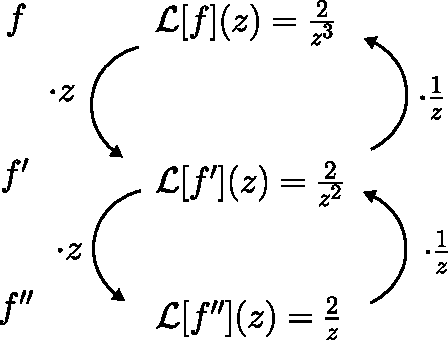
\includegraphics[width=0.4\textwidth]{figure/2026-04-23.pdf}
\caption{Laplace transform of polynomials}
\end{figure}
\begin{parag}{$ $}
    Which confirms our previous computations. Note carefully we used $f\left(0\right) =  f'\left(0\right) = 0$
\end{parag}



\begin{theoreme}
Let $f : \mathbb{R}_+ \to \mathbb{C}$ piecewise continuous and $\gamma_0 \geq 0$ an abscissa of convergence for $f$. Define $g: \mathbb{R}_+ \to \mathbb{C}$ by $g\left(t\right) = \int_0^{t}f\left(s\right)ds$. Then when $\text{Re }z > \gamma_0$,
\begin{align*} 
	\mathcal{L}\left[g\right]\left(z\right) = \frac{1}{z}\mathcal{L}\left[f\right]\left(z\right)
\end{align*}
\end{theoreme}

\begin{framedremark}
In general the abscissa of convergence for $g$ cannot be negative. (even if it is for $f$).
\end{framedremark}


\begin{proof}
    Note $g' = f$ and $g\left(0\right) = 0$. By the previous theorem,
	\begin{align*} 
		\mathcal{L}\left[f\right]\left(z\right) = \mathcal{L}\left[g'\right]\left(z\right) = z \mathcal{L}\left[g\right]\left(z\right) - \underbrace{g\left(0\right)}_{= 0}\\
	\end{align*}
	Therefore we have 
	\begin{align*} 
		\mathcal{L}\left[g\right]\left(z\right) = \frac{1}{z}\mathcal{L}\left[f\right]\left(z\right)
	\end{align*}
\end{proof}
(We will not show why $\mathcal{L}\left[g\right]\left(z\right)$ is indeed defined for $\text{Re }z \geq \gamma_0$ when $\gamma_0 \geq 0$)



\begin{theoreme}
Let $a > 0$ and $b \in \mathbb{R}$. Let $f : \mathbb{R}_+ \to \mathbb{C}$ piecewise continuous with an abscissa of convergence $\gamma_0 \in \mathbb{R}$. Define $g : \mathbb{R}_+ \to \mathbb{C}$ by $g\left(t\right) = e^{-bt}f\left(at\right)$. Then
\begin{align*} 
	\mathcal{L}\left[g\right]\left(z\right) = \frac{1}{a}\mathcal{L}\left[f\right]\left(\frac{z + b}{a}\right)
\end{align*}
	This hold in essence when the right hand side exists, and this is the case when $\text{Re } \frac{z + b}{a} > \gamma_0$ (which is equivalent to $\text{Re }z > a \gamma_0 - b$ because $a > 0$ and $b \in \mathbb{R}$)\\
	$ $\\
	In fact: $a \gamma_0 - b$ is an abscissa of convergence for $g$
\end{theoreme}
\begin{proof}
    By the definition we have that 
	\begin{align*} 
		\mathcal{L}\left[g\right]\left(z\right) &=  \int_0^{\infty}e^{-bt}f\left(at\right)e^{-zt}dt\\
		&=  \int_0^{\infty}f\left(at\right) e^{-\left(z + b\right)t}dt 
	\end{align*}
	So here in order to have the same transformation as the one for $f$ we have to get rid of the $a$ in the argument, we can do so using substitution. Let $s = at$ and $ds =  adt$. As we know that $a > 0$ we can rewrite our integral as
	\begin{align*} 
		&=  \int_0^{\infty}f\left(s\right) e^{-z + b}\frac{S}{a}\frac{ds}{a}\\
		&= \frac{1}{a}\int_0^{\infty}f\left(s\right)e^{-\frac{zt + b}{a}s}ds = \frac{1}{a}\mathcal{L}\left[f\right]\left(\frac{z + b}{a}\right)
	\end{align*}
\end{proof}


\begin{parag}{Example}
    Let us have $g\left(t\right) = e^{ct}= e^{ct} \cdot  1$. Using the fact that the Laplace transform of $1$ is $\frac{1}{z}$ we can use the theorem stated above in order to find the Laplace transform of $g$. Here $a = 1, b =  -c$. By the theorem, where $\text{Re }z > -b = c$ we have 
	\begin{align*} 
		\mathcal{L}\left[g\right]\left(z\right) =  \mathcal{L}\left[1\right]\left(z - c\right) = \frac{1}{z - c}
	\end{align*}

\end{parag}



\begin{framedremark}
The fact that $c$ is an abscissa of convergence for $g$ can be shown by hand, without relying on the above theorem.
\end{framedremark}



\begin{parag}{Example}
	Find $f : \mathbb{R}_+ \to \mathbb{C}$ such that $\mathcal{L}\left[f\right]\left(z\right) = \frac{1}{\left(z - a\right)\left(z - b\right)}$ where $a, b \in \mathbb{R}$. To do so we will divide our transform into sum of fraction as in the previous example. Then using the linearity of the Laplace transformation we will be able to find our function.
	\begin{align*} 
		\mathcal{L}\left[f\right]\left(z\right) &= \frac{1}{b-a} \left[\frac{1}{z-b} - \frac{1}{z-a}\right]\\
												&=	\frac{1}{b-a}\left[\mathcal{L}\left[e^{bt}\right]\left(z\right) - \mathcal{L}\left[e^{at}\right]\left(z\right)\right]\\
												&= \mathcal{L}\left[\frac{e^{bt} - e^{at}}{b-1}\right]\left(z\right)
	\end{align*}
	This is defined when the two Laplace transforms in the middle are both defined, when $\text{Re }z > \max \left\{a, b\right\}$.
\end{parag}




\begin{parag}{Convolution}
    Let $f, g : \mathbb{R}_+ \to \mathbb{C}$ functions that are piecewise continuous. By extending those functions by $0$ on $\left(-\infty, 0\right)$. We can again defined the convolution as we did in previous section 
	\begin{align*} 
		f \ast g\left(t\right) &= \int_{-\infty}^{\infty}f\left(t-s\right)g\left(s\right)ds = \begin{cases}
			\int_{0}^{t}f\left(t-s\right)g\left(s\right)ds \mathspace \mathspace t > 0\\
			0 \mathspace \mathspace \mathspace\text{ otherwise}
		\end{cases}
	\end{align*}
	The reason for the case is that we can cut out bornes on our integral. Notice that $g\left(s\right) = 0$ when $s < 0$ therefore all the interval $\left(-\infty, 0\right)$ doesn't have any effect on the result of our integral (as $f\left(t- s\right)g\left(s\right) = 0$ there). Also, when $s > t$, the argument of $f$ becomes negative which also makes the value integrated $0$. Therefore only when $s \in \left(0, t\right)$ we have a non trivial contribution to our integral.\\
	$ $\\
	In particular $f \ast g$ can be restricted back to $ \mathbb{R}_+$ since its values on $\left(-\infty, 0\right)$ are trivial. That way we can regard $f \ast g : \mathbb{R}_+ \to \mathbb{C}$ and compute its Laplace transform.
\begin{theoreme}
Let $f, g: \mathbb{R}_+ \to \mathbb{C}$ piecewise continuous with common abscissa of convergence $\gamma_0 \in \mathbb{R}$. Then $\gamma_0$ is an abscissa of convergence for $f\ast g$ and when $\text{Re }z > \gamma_0$ 
\begin{align*} 
	\mathcal{L}\left[f \ast g \right]\left(z\right) = \mathcal{L}\left[f\right]\left(z\right) \mathcal{L}\left[g\right]\left(z\right)
\end{align*}
\end{theoreme}
\end{parag}




